\documentclass[11pt]{article}
\usepackage{latexsym}
\usepackage{amsmath}
\usepackage{amssymb}
\usepackage{amsthm}
\usepackage{epsfig}
\usepackage[tight]{subfigure}
\usepackage{cases}
\usepackage{amsmath}

\DeclareMathOperator*{\minimize}{min}
\DeclareMathOperator*{\maximize}{max}

\usepackage{algorithm}
 %on linux you may need to run sudo apt-get install texlive-full to install algorithm.sys
\usepackage{algorithmic}

\usepackage{verbatim}

\newcommand{\handout}[5]{
  \noindent
  \begin{center}
  \framebox{
    \vbox{
      \hbox to 5.78in { {#1} \hfill #2 }
      \vspace{4mm}
      \hbox to 5.78in { {\Large \hfill #5  \hfill} }
      \vspace{2mm}
      \hbox to 5.78in { {\em #3 \hfill #4} }
    }
  }
  \end{center}
  \vspace*{4mm}
}

\newcommand{\lecture}[5]{\handout{#1}{#2}{#3}{#4}{#5}}
\newcommand{\collision}[0]{\mathrm{collision}}
\newcommand{\nocollision}[0]{\overline{\collision}}

\newcommand*{\QED}{\hfill\ensuremath{\square}}

\newtheorem{theorem}{Theorem}
\newtheorem{corollary}[theorem]{Corollary}
\newtheorem{lemma}[theorem]{Lemma}
\newtheorem{observation}[theorem]{Observation}
\newtheorem{proposition}[theorem]{Proposition}
\newtheorem{definition}[theorem]{Definition}
\newtheorem{claim}[theorem]{Claim}
\newtheorem{fact}[theorem]{Fact}
\newtheorem{assumption}[theorem]{Assumption}
\newtheorem{note}[theorem]{Note}

% 1-inch margins, from fullpage.sty by H.Partl, Version 2, Dec. 15, 1988.
\topmargin 0pt
\advance \topmargin by -\headheight
\advance \topmargin by -\headsep
\textheight 8.9in
\oddsidemargin 0pt
\evensidemargin \oddsidemargin
\marginparwidth 0.5in
\textwidth 6.5in

\parindent 0in
\parskip 1.5ex
%\renewcommand{\baselinestretch}{1.25}

\begin{document}

\lecture{Statistical Techniques in Robotics (16-831, S21)}{Lecture \#11
  (Wednesday, March 10)}{Lecturer: Kris Kitani}{Scribes: Jinkun Cao, Yuda Song}{AdaBoost \& MAB}

\section{Review}
In the last lectures, on the problem of supervised learning, we studied some online technique SVM, i.e. Support Vector Machine. Online techniques can be very useful for supervised learning. Different from the usual supervised learning, online learning interweaves the training and testing steps.

\begin{figure}[H]
    \centering
    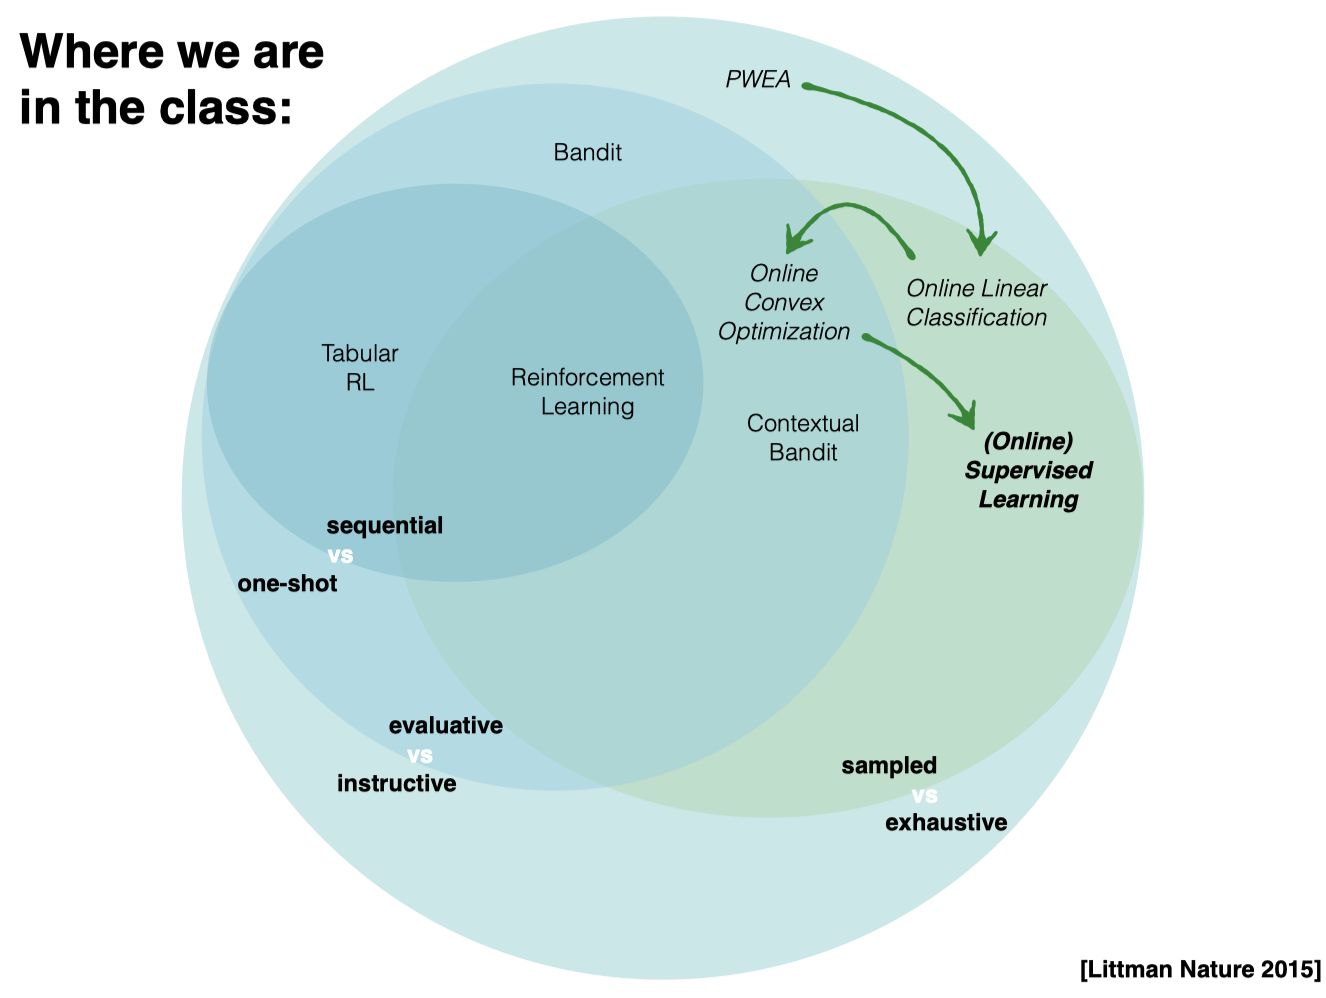
\includegraphics[width=.6\linewidth]{lecture_11_B/figs/SVM_arch.png}
    \caption{Where the online supervised learning is categroied.}
    \label{fig:cate}
\end{figure}

\subsection{Support Vector Machine (SVM)}

\subsubsection{Hyperplanes}
To have a good classifier, we basically want to find a proper hyperplane to divide data points into different ``regions''. A hyperplane is a subspace whose dimension is one less than that of its ambient space. If a space is 3-dimensional then its hyperplanes are the 2-dimensional planes, while if the space is 2-dimensional, its hyperplanes are the 1-dimensional lines\footnote{https://en.wikipedia.org/wiki/Hyperplane}. A common example for the most seen 1D and 2D hyperplanes are shown in Figure~\ref{fig:2d_plane}
 and Figure~\ref{fig:3d_plane}.
\begin{figure}[H]
    \centering
    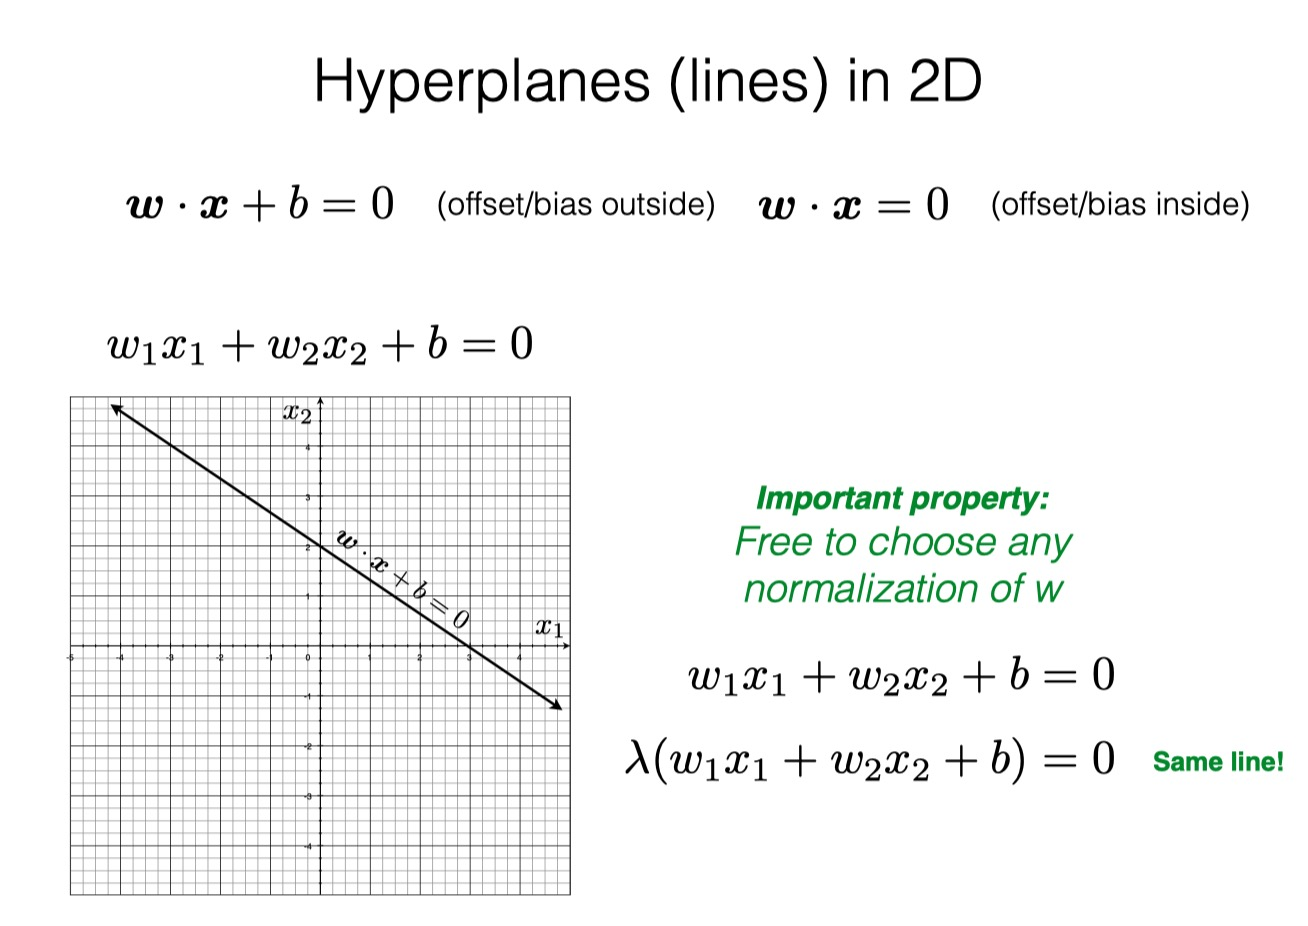
\includegraphics[width=.6\linewidth]{lecture_11_B/figs/2d_plane.png}
    \caption{A hyperplane in 2D space is just an 1D line.}
    \label{fig:2d_plane}
\end{figure}

\begin{figure}[H]
    \centering
    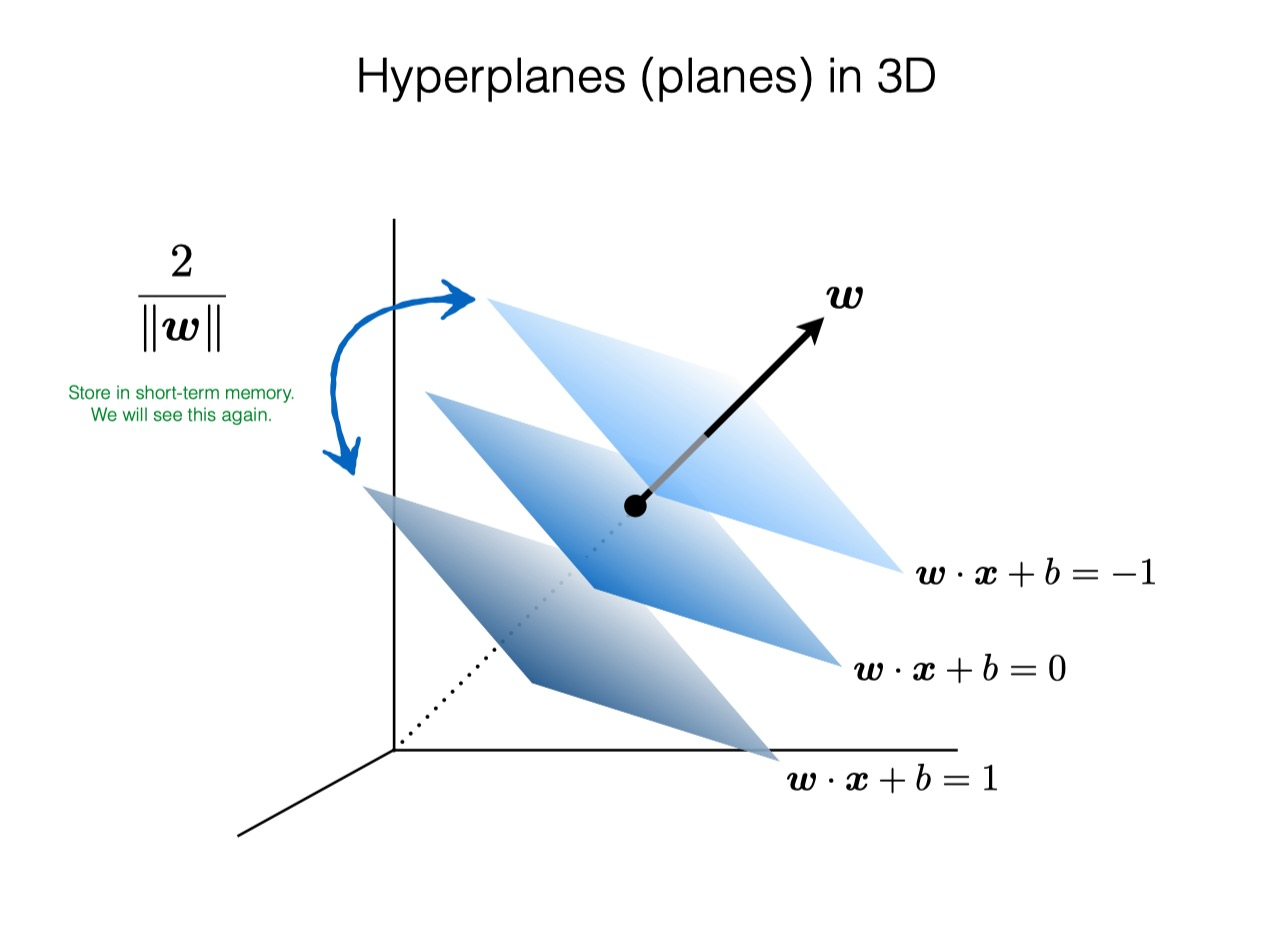
\includegraphics[width=.6\linewidth]{lecture_11_B/figs/3d_plane.png}
    \caption{A hyperplane in 3D space is just an 2D plane.}
    \label{fig:3d_plane}
\end{figure}

\subsubsection{Support Vector Machine}
A Support Vector Machine (SVM)~\cite{noble2006support} is basically a max-margin classifier. It aims to find a hyperplane in the data space to divide data points into categories they belong to. And the optimization objective is usually to maximize the margin between data points and the hyperplane boundary. Consider we describe the hyperplane with 

\begin{equation}
    \mathbf{w} \cdot \mathbf{x} + b = 0,
\end{equation}

and the points that most close to the plane on two sides are located on the hyperplane $\mathbf{w} \cdot \mathbf{x} + b = 1$ and $\mathbf{w} \cdot \mathbf{x} + b = -1$. Then, for the two-class classification setting, we can formulate the objective as a maximization problem, for $i=1,...,N$, 

\begin{numcases}{max_{\mathbf{w}} \frac{2}{||\mathbf{w}||}, \quad s.t. \quad \mathbf{w} \cdot \mathbf{x}_i + b \quad}
      \ge +1  if y_i = +1 \\
      \leq -1 if y_i = -1 .
\end{numcases} 

So it is equivalent to find 

\begin{equation}
    min_{\mathbf{w}} || \mathbf{w} ||^2, \quad s.t. \quad y_i (\mathbf{w} \cdot \mathbf{x}_i + b ) \ge 1  ( i = 1,..., N),
\end{equation}

which is a convex quadratic programming problem, so there exists a unique solution.

\subsubsection{‘Soft’ Margin SVM}
In practice, there might be some situations where we can not find a hyperplane to divide points of different categories into different sides perfect or there exists only extremely narrow margin if we force such a ``perfect'' classification which might lead the solution less robust because of overfitting. So intuitively, we should allow for some misclassification if we can get more robust classification. Under such a philosophy, we actually make a trade-off between the \textbf{MARGIN} and the \textbf{MISTAKES}. To realize this, we add a slack variable $\xi$, making the constrain,

\begin{equation}
    y_i (\mathbf{w}^T \mathbf{x}_i + b ) \ge 1 - \xi_i.
\end{equation}

By allowing the slackness, we convert the original SVM into the `soft' margin SVM. The objective is converted to 

\begin{equation}
    min_{\mathbf{w}, \xi} || \mathbf{w} || ^2 + C \sum_i \xi_i,
\end{equation}

where $C$ is a regularization parameter that a small $C$ tends to ignore the constrain to find a large margin while a big $C$ tends to emphasize the effect of constrain. By adding the slackness, the optimization objective still forms a quadratic programming problem, thus an unique solution exists. A illustration of 'Soft' Margin SVM is shown in Figure~\ref{fig:soft_svm}. 

\begin{figure}[H]
    \centering
    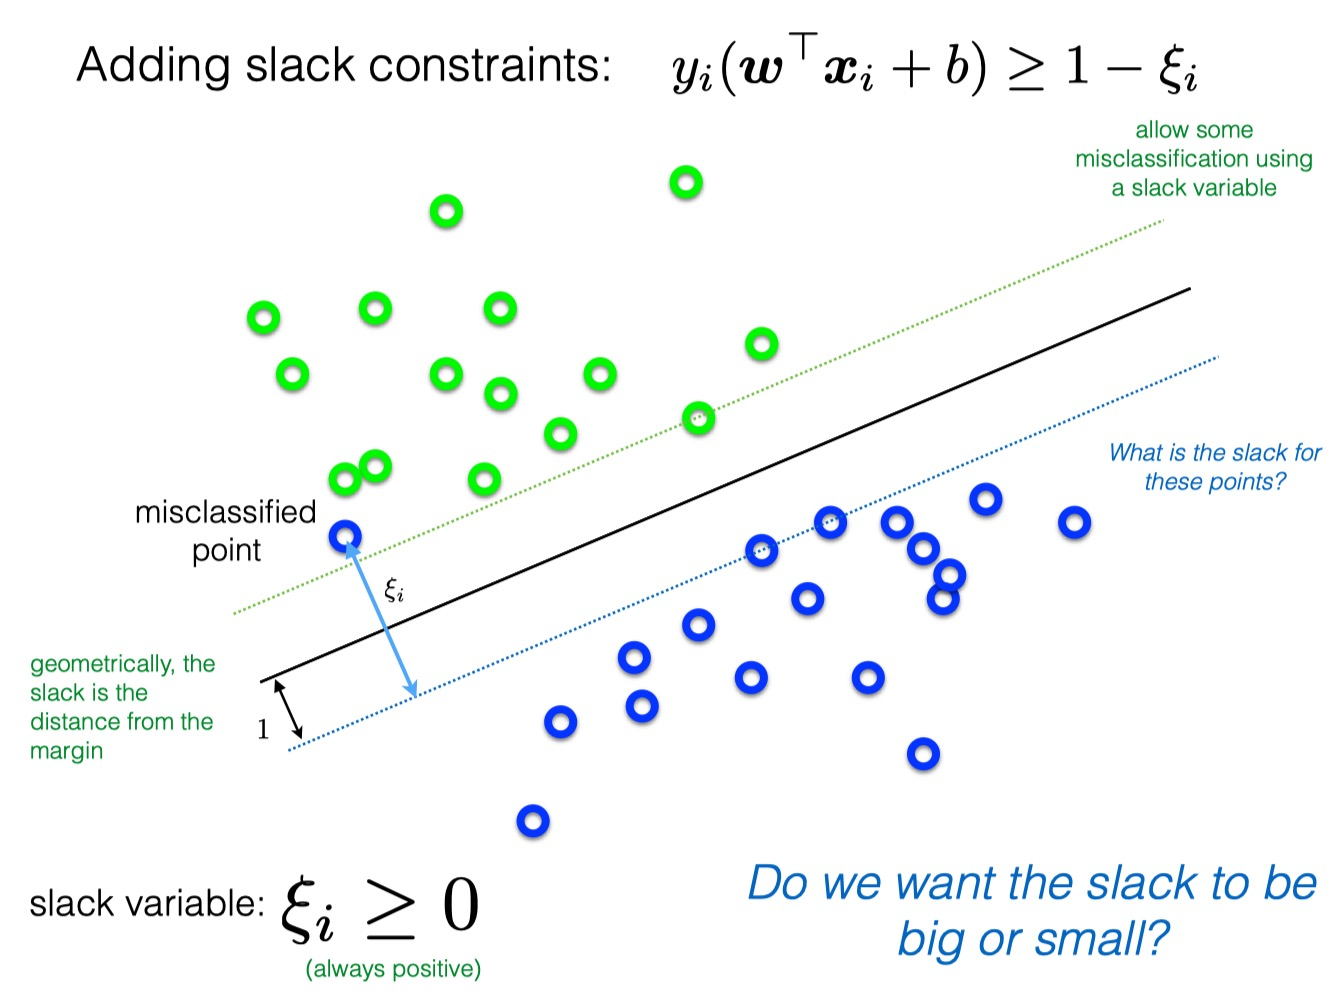
\includegraphics[width=.5\linewidth]{lecture_11_B/figs/slack.png}
    \caption{When adding slackness into SVM, we allow some misclassification to make the solution more robust.}
    \label{fig:soft_svm}
\end{figure}

Finally, by combining the regularization and loss function, we have an adaptive optimization object 

\begin{equation}
    min_{\mathbf{w}} (\frac{\lambda}{2} || \mathbf{w} ||^2 + \frac{1}{M} \sum_{m=1}^M max \{0, 1- y_m\mathbf{w}^T \mathbf{x}_m\}),
\end{equation}

which is convex but not differentiable. Hence, to solve the problem, we use Sub-Gradient Descent instead of the Gradient Descent we have been familiar with. A subgradient\footnote{https://www.stat.cmu.edu/~ryantibs/convexopt-F15/lectures/06-subgradients.pdf} for a convex function $f$ at $x$ is any $g \in \mathbb{R}^n$ such as 

\begin{equation}
    f(y) \ge f(x) + g^T  (y-x).
\end{equation}

For the hinge loss, we have its subgradient expression as 

\begin{numcases}{z_m = }
      \mathbf{0}, \quad y_m \mathbf{w}^T \mathbf{x}_m \ge 1 \\
      -y_m \mathbf{x}_m, \quad otherwise.
\end{numcases} 

So come to here, we could write the algorithm of soft margin SVM as in Algorithm \ref{algo:soft_svm}.

\begin{algorithm}[H]
\caption{Soft SVM}
\label{algo:soft_svm}
\begin{algorithmic}[1]
\STATE $\theta^{(1)} \longleftarrow 0 \in \mathbb{R}^N$
\FOR{t=1,...,T }
\STATE $y_d, x_d \sim D$
\STATE $\theta^{(t)} = \theta^{(t-1)} + y_d x_d \cdot \mathbf{1}[y_d (\mathbf{w}^{(t)} \cdot \mathbf{x}_d) < 1]$
\STATE $\mathbf{w}^{(t+1)} \longleftarrow \frac{1}{\lambda(t+1)} \theta^{(t)}$
\ENDFOR
\STATE $\bar{\mathbf{w}} = \frac{1}{T} \sum_t \mathbf{w}^t$
\end{algorithmic}
\end{algorithm}


\section{PAC Learning}

PAC Learning~\cite{valiant1984theory}, short for ``Probably Approximately Correct Learning'', is a theoretical framework for answering the question: \textbf{What is the optimal dataset size to obtain good generalization?}

To explain the learning framework, we need some terminology first. When a dataset $D$ of size $N$ is drawn from a distribution $P(x,y)$ and the class labels are determined by an unknown deterministic distribution $y = f^\star(x)$. Then for a single classifier, we could denote a function $f$ drawn from space of function $\mathcal{F}$ and obtained by training on the training data, so we have 

\begin{equation}
    f(x;D) \sim \mathcal{F} | D.
\end{equation}

For a learned function $f$, it has good generalization if its expected error rate is below a pretrained value 

\begin{equation}
E_{p(x,y)} [\mathbf{1}[f(x;D)\neq y]] < \epsilon.
\label{eq:error}
\end{equation}

Under these backgrounds, a PAC learning algorithm requires that the inequality \ref{eq:error} holds with probility $1 - \sigma$, where $\epsilon$ is defined to define a ``approximately correct''. Broadly, there are two types of PAC learning algorithms: Strong PAC-learning and Weak PAC-learning.

\paragraph{Strong PAC-learning Algorithm.} Given $\epsilon$, $\sigma$ and $D \sim P(x,y)$, learner outputs with probability $1-\sigma$ a hypothesis (function) with error at most $\epsilon$.

\paragraph{Weak PAC-learning Algorithm.} Given $\epsilon$, $\sigma$ , $D \sim P(x,y)$ and $\gamma > 0$, learner outputs with probability $1-\sigma$ a hypothesis (function) with error at most $\epsilon \ge 1/2 - \gamma$.

For both strong and weak PAC-learning algorithms, the run time must to polynomial in $1/\sigma$ and $1/\epsilon$ and other relevant parameters such as the size of the examples or complexity of the target concept. 

Then, the key point is ... \textbf{Any weak learning algorithm can be boosted into a strong learning algorithm}~\cite{schapire1990strength}.


\section{AdaBoost}
To have a stronger PAC learner by boosting from weak learners, the basic strategy is to \textbf{call a weak PAC learner multi times (generates a sequence of hypothesis), but at each time, present it with a different distribution $D$. Then combine all hypothesis into a single hypothesis (strong PAC learner).}

Following the philosophy, AdaBoost~\cite{freund1997decision}, short for ``Adaptive Boosting'', it is a machine learning to be used in conjunction with other types of learning algorithms to improve (boost) performance. The output of the other learning algorithms is combined into a weighted sum that represents the final output of the boosted version of classifier~\footnote{https://en.wikipedia.org/wiki/AdaBoost}. The algorithm of AdaBoost is presented in Algorithm~\ref{algo:adaboost}. Where line 3-4 are for prediction from the weak learner and line 5-7 are for update parameters.

\begin{algorithm}[H]
\caption{AdaBoost}
\label{algo:adaboost}
\begin{algorithmic}[1]
\REQUIRE $D=\{x_n, y_n\}_{n=1}^N$, $\{w_n^{(0)}\}_{n=1}^N$, $T$
\FOR{t=1,...,T }
\STATE $\mathbf{p}^{(t)} = \mathbf{w}^{(t-1)} / \sum_{n} w_n^{(t-1)}$
\STATE $h^{(t)} = $ WEAKLEARNER $(D, \mathbf{p}^{(t)})$
\STATE $\epsilon^{(t)} = \sum_n p_n^t | h^{(t)} (x_n) - y_n | $
\STATE $\beta^{(t)} = \epsilon^{(t)} / 1 - \epsilon^{(t)}$
\STATE $w_n^{(t)} = w_n^{(t-1)} \beta^{1 - |h^{(t)} (x_n^{(t)}) -y_n^{(t)} |} \forall n$
\ENDFOR
\STATE $h_F(x) = \mathbf{1}[\sum_{t=1}^T (log \frac{1}{\beta^{(t)}}) h^{(t)} (x) \ge \frac{1}{2} \sum_{t=1}^T (log \frac{1}{\beta^{(t)}})]$
\end{algorithmic}
\end{algorithm}

Within the algorithm, we should pay attention to some important components. $\mathbf{p}^{(t)}$ is the probability distribution over the data items. It is used to re-weight the training dataset then more weight is assigned to ``important/hard'' data items. $h^{(t)}$ is the hypothesis or classifier returned by a weak learning algorithm. Then, for the update part, $\epsilon^{(t)}$ is the average error/loss of the obtained hypothesis in the prediction stage. $\beta^{(t)}$ is the penalty constant to judge a classifier. For example, when the classifier is good, $\beta$ should approach 0 or it approaches infinity if the classifier is bad. Finally, in line 6, the weight is updated in a manner of exponential update. Line 8 in the algorithm gives the final hypothesis after boosting where it contains an inequality of which the LHS is the weighted combination of hypothesis and the RHS is the weight total. 

With this AdaBoost algorithm, the error bound is essentially 
\begin{equation}
    \epsilon \leq w^T \Pi_{t=1}^T \sqrt{\epsilon_t (1-\epsilon_t)}.
\end{equation}

\section{Multi-Armed Bandit}
We then come to the area of solving Multi-Armed Bandit problem where a fixed limited set of resources must be allocated between competing (alternative) choices in a way that maximizes their expected gain, when each choice's properties are only partially known at the time of allocation, and may become better understood as time passes or by allocating resources to the choice~\footnote{https://en.wikipedia.org/wiki/Multi-armed\_bandit}. The concept of Multi-Armed Bandit problem is essentially explained in the Veen Diagram of Figure~\ref{fig:MAB}.

\subsection{Introduction}
Basically, for a typical Multi-Armed Bandit, we have multiple bandit machines, each of which has an unknown reward distribution. We are allowed to pull one arm among them to get a reward each time. We need to carefully select which arm to pull next to maximize the total reward over a time interval or $T$ decisions. MAB problem has

\begin{itemize}
    \item one-shot feedback, as one action leads to one reward where selecting an action does not change the state of the next time step;
    \item exhaustive feedback, as the 'state' is static and finite because there is no state and actions are finite. A player could pull all arms over the duration of the game;
    \item evaluative feedback, as we receive a sampled reward at each time step.
\end{itemize}

\begin{figure}[H]
    \centering
    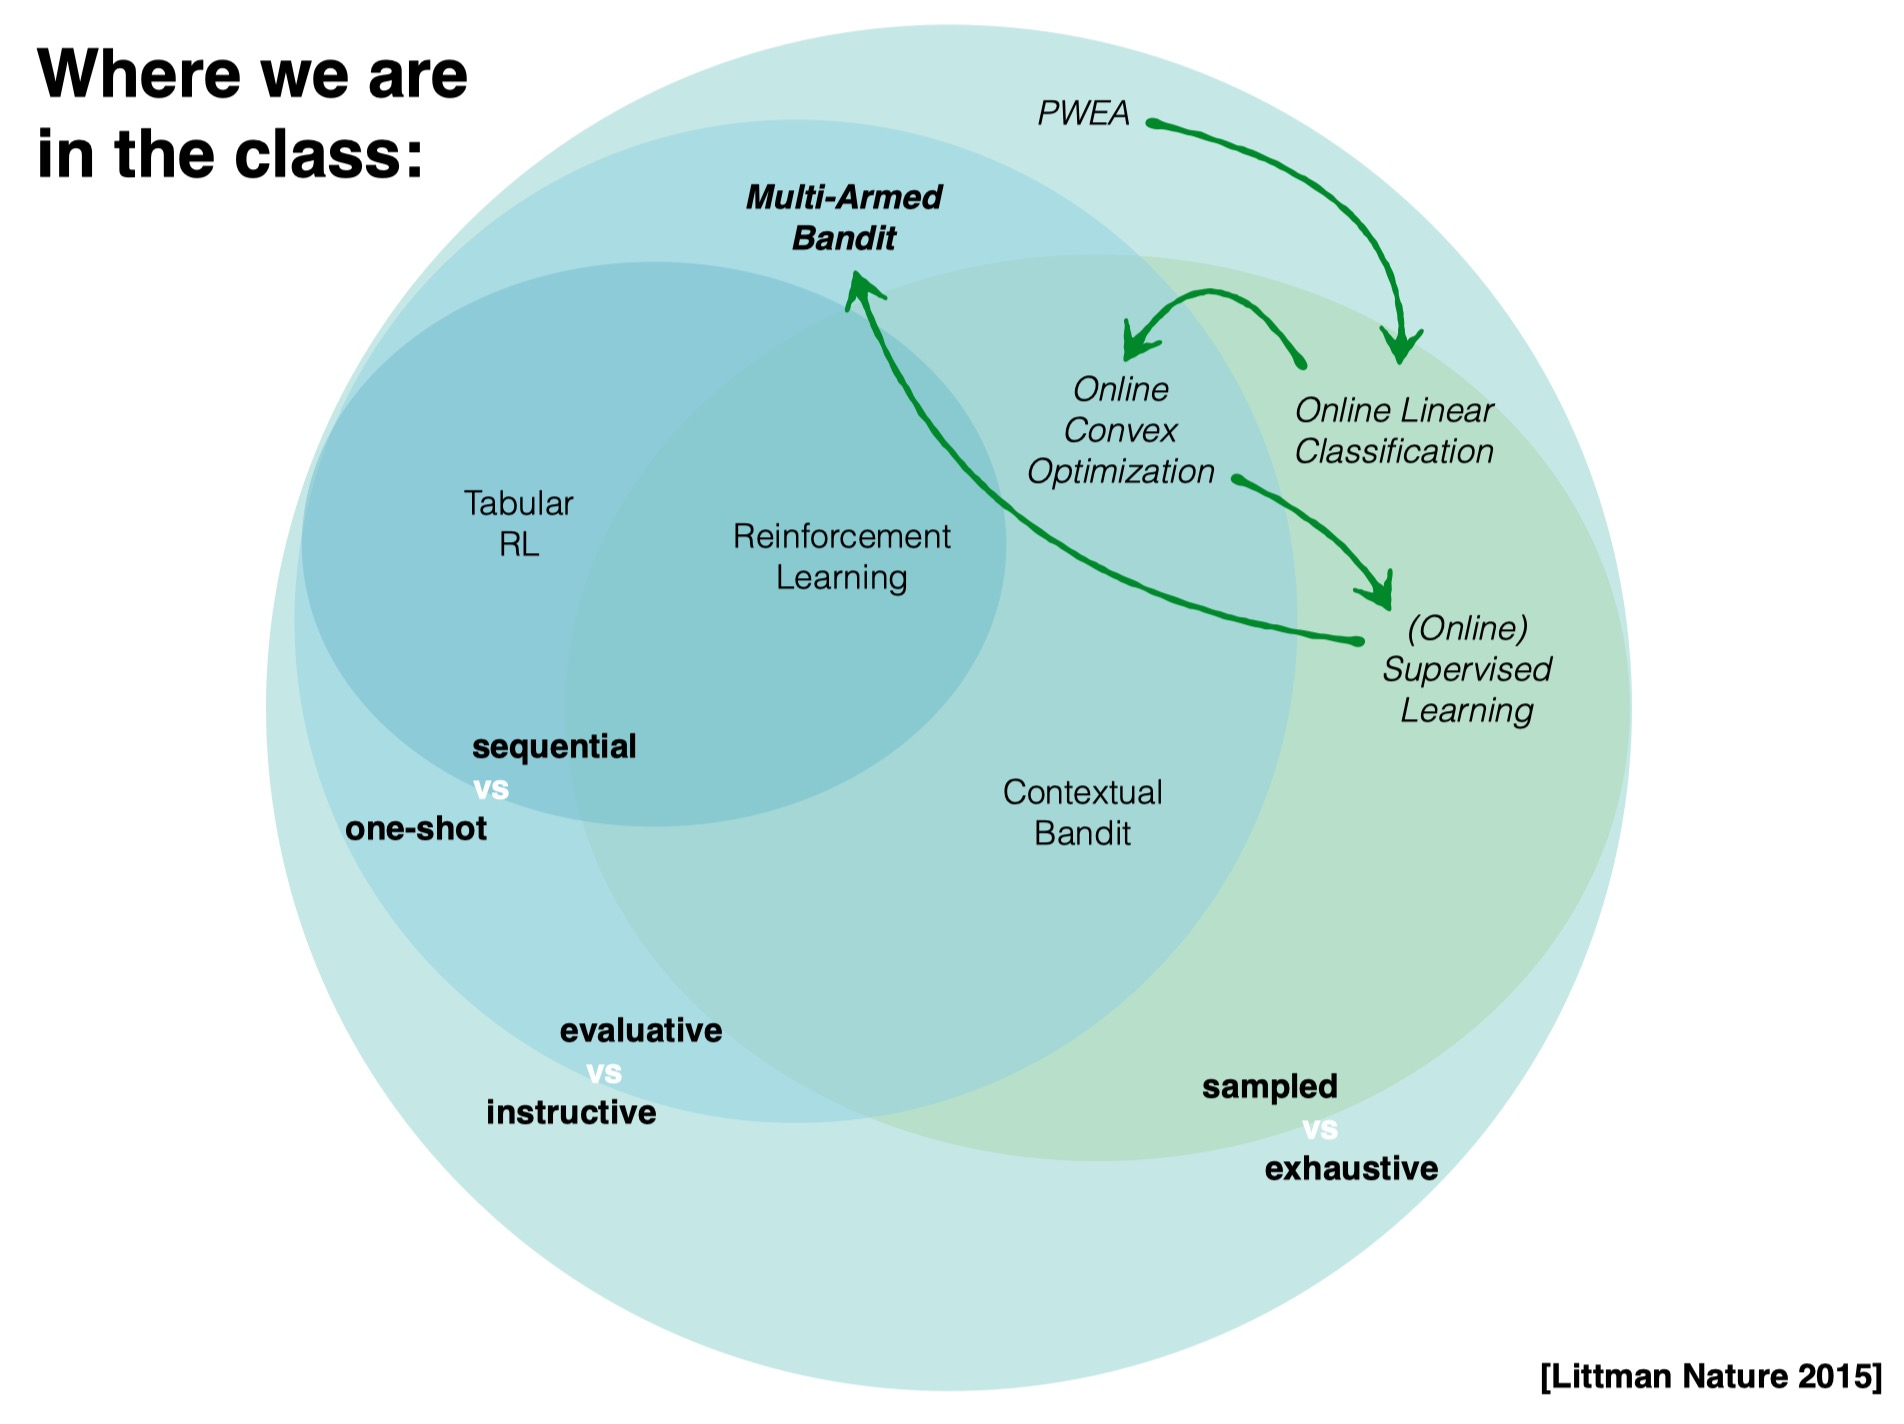
\includegraphics[width=.7\linewidth]{lecture_11_B/figs/multiarm_bandit.png}
    \caption{Where the Multi-Armed Bandit problem is in the Concept Venn Diagram.}
    \label{fig:MAB}
\end{figure}

In previous tasks, we usually study the loss from an action $l_t \in [0,1]$, now we can rewrite it as a reward $g_t = 1 - l_t \in [0,1]$. Then the regret now becomes

\begin{equation}
    R^{(T)}(h) = \underbrace{\sum_{t=1}^T g(h(x^{(t)}), y^{(t)})}_{\text{reward of a hypothesis (expert)}} - \underbrace{\sum_{t=1}^T g(\hat{y}^{(t)}, y^{(t)})}_{\text{reward of the online algorithm}}.
\end{equation}

\subsection{Exploration-Exploitation}
Different from PWEA situation, where we have full loss observation, we only have partial loss observability in bandit problem. It says that learner observes loss only for their action. So, we need to explore what the feedback might be if we take different actions, which leads to an Exploration-Exploitation solution naturally. Because we need to \textbf{explore arms that might do well in the future} and \textbf{exploit arms that did well in the past.} We note here that this solution is proposed under the \textbf{Stochastic Bandits} environments~\cite{robbins1952some} where (1) each arm has a static reward distribution and (2) each pull gives a sample from a distribution. The process of Explore-Exploit under careful balance of the tradeoff of exploration and exploitation is shown in Algorithm~\ref{algo:exp2}.

\begin{algorithm}[H]
\caption{Explore-Exploit}
\label{algo:exp2}
\begin{algorithmic}[1]
\REQUIRE $M$
\FOR{$k=1,\;\cdots,\;K$}
\FOR{$m=1,\;\cdots,\;M$}
\STATE $a = k$
\STATE $\text{Receive}(r)$
\STATE $\widehat{\mu}_k = \widehat{\mu}_k + \frac{r}{M}$
\ENDFOR
\ENDFOR
\FOR{$t=KM,\;\cdots,\;T$}
\STATE $a^{(t)} = \arg\max_{k}\widehat{\mu}_k'$
\ENDFOR
\end{algorithmic}
\end{algorithm}

And the regret bound for Explore-Exploit is 

\begin{equation}
    R_{\text{explore-exploit}} = \mathcal{O}(K^{1/3}T^{2/3}).
\end{equation}


{
\bibliography{lec11refs}
\bibliographystyle{abbrv}
}

\newpage
\section{Appendix}
We provide some materials here which might be interesting to read and highly related to this lecture. 

\subsection{More for SVM}
Despite the elegant form of SVM algorithms, it is hard to solve it in many real scenes, when, for example, the data scattering is messy to obtain good enough hyperplane with convincing margin or the data volume is too large to design efficient solver and so on. To tackle these real-world problems, many researchers have provided great progress in the application of SVM. 

An early paper~\cite{joachims1998making} focuses on the quadratic optimization problem with bound constraints and one linear equality that training a SVM leads to. From this reason, large learning tasks with many training examples on the shelf optimization techniques for general quadratic programs quickly become intractable in their memory and time requirements. Authors of this paper designed a system to solve large-scale SVM training in an efficient manner.  

Another work~\cite{cherkassky2004practical} continues to investigate practical selection of hyper-parameters for support vector machines (SVM) regression (that is, $\epsilon$-insensitive zone and regularization parameter $C$ we introduced in this lecture). The proposed methodology advocates analytic parameter selection directly from the training data, rather than re-sampling approaches commonly used in SVM applications. They also prove the good generalization ability of the proposed scheme.

A more recent work~\cite{shalev2011pegasos} makes a breakthrough on solving SVM more quickly. They describe and analyze a simple and effective stochastic sub-gradient descent algorithm for solving the optimization problem cast by Support Vector Machines (SVM). We prove that the number of iterations required to obtain a solution of accuracy $\epsilon$ is  $\mathcalO{O}(1/\epsilon)$ , where each iteration operates on a single training example. In contrast, previous analyses of stochastic gradient descent methods for SVMs require $\Omega (1/\epsilon^2)$  iterations. 

%As a classic machine learning algorithm, SVM has been beaten by many more modern machine learning or even deep learning solutions on broad problems. But even for the most advanced research SVM is still providing active inspiration. The combination of SVM and recently popular deep learning is actually worth to pay attention to. 

\subsection{More for Multi-Armed Bandits}
On a broad range of Multi-Armed Bandits, there are actually diverse works analysing solution complexity, performance bound and proposing new solutions. 

\subsubsection{More Analysis}
A very famous paper~\cite{bubeck2012regret} focuses on two extreme cases in which the analysis of regret of MAB problem is particularly simple and elegant: i.i.d. payoffs and adversarial payoffs. Besides the basic setting of finitely many actions, they also analyze some of the most important variants and extensions, such as the contextual bandit model. More recently, a work~\cite{vermorel2005multi} studies the performance of existing solutions for Multi-Armed Bandits in an empirical perspective.

From the perspective of KL divergence, a previous work~\cite{maillard2011finite} proposes a finite-time analysis of Multi-armed Bandits Problems, whose conclusion agrees with previous analysis from different perspectives. 

\subsubsection{More applications}
Besides, for some special cases of MAB problem, there are also some interesting works. For example, for the generalization of single-armed bandit problem to the classic subset selection problem, a previous work~\cite{kalyanakrishnan2012pac} addresses and analyses it pretty well. It gives a novel expected sample complexity bound for subset (and single-arm) selection.
They have also given a worst case sample complexity
lower bound for subset selection.

Some literature also tries to combine other tools with existing knowledge in this area. For example, a recent paper~\cite{scott2010modern} tries to leverage Bayesian computation in this area. As the  advances in Bayesian computation have made randomized probability matching easy to apply to virtually any payoff distribution. This flexibility frees the experimenter to work with payoff distributions that correspond to certain classical experimental designs that have the potential to outperform methods that are ‘optimal’ in simpler contexts. in this paper, the authors summarize the relationships between randomized probability matching and several related heuristics. And its context is pretty modern that the focus is mainly on the application in reinforcement learning. 

%\section{Appendix}
%This section provides any relevant background material that was not covered in the lectures, but was found to be useful for understanding the material. 
%For example, derivations, theory underlying techniques employed, etc. 

%Additionally, this section can summarizes applications or extensions of these techniques found in the literature. 

\end{document} % Done!


